% ===========================================================================
% Chapter 1 — Blockchain Fundamentals
% Study Guide: Blockchain & Cardano Credential Verification
% ===========================================================================

% ---- Shared TikZ style definitions for this guide -------------------------
\tikzset{
  guidebox/.style={draw, rounded corners=4pt, thick, align=center,
                   font=\sffamily\small, fill=white, minimum height=1cm},
  guidearrow/.style={-{Latex[length=2.5mm]}, thick, color=gray!70!black},
  guidelabel/.style={font=\sffamily\footnotesize, text=gray!50!black},
}

% Convenience colours (semantic names for repeated fills)
\colorlet{inputcolor}{blue!8}
\colorlet{processcolor}{green!8}
\colorlet{outputcolor}{orange!8}
\colorlet{blockchaincolor}{purple!8}
\colorlet{securitycolor}{red!6}
\colorlet{intermediatecolor}{yellow!8}
\colorlet{neutralcolor}{gray!10}

% ===================================================================
\chapter{Blockchain Fundamentals}
\label{ch:blockchain-fundamentals}
% ===================================================================

This chapter introduces the foundational concepts you need before we touch a
single line of Cardano code.  Every idea is explained from scratch---no prior
knowledge of blockchain, cryptography, or distributed systems is assumed.  By
the end of this chapter you will understand \emph{what} a blockchain is,
\emph{why} it works, and \emph{how} Cardano improves on earlier designs.
These building blocks are essential for the credential-verification system we
will construct in later chapters.

% -------------------------------------------------------------------
\section{What Is a Blockchain?}
\label{sec:what-is-blockchain}
% -------------------------------------------------------------------

Imagine a notebook that sits in the centre of a town square.  Every time
someone makes a deal---say, Alice sells a bicycle to Bob---they walk to the
square and write the transaction in the notebook for everyone to see.  Once a
page is full, a town clerk stamps it with a unique seal, tears it out, and
staples it to the previous page.  The seal on each new page includes a
reference to the seal on the page before it.  If anyone tried to rip out a
page in the middle and replace it, the seals would no longer match and the
entire town would immediately notice.

A \textbf{blockchain} is the digital version of that notebook.  Instead of
pages we have \emph{blocks}; instead of a staple we have a
\emph{cryptographic hash} (explained in Section~\ref{sec:hashing}); and
instead of one notebook in a square, thousands of identical copies are
maintained by computers all over the world.

\subsection{Blocks}

A \textbf{block} is a bundle of data.  In a financial blockchain the data is
a list of transactions (``Alice sent 10 tokens to Bob''), but blocks can hold
any kind of information---credential issuances, votes, supply-chain events,
or software licence grants.  Every block also carries a small header that
contains bookkeeping metadata: a timestamp, a reference to the previous
block, and the result of running all the block's data through a hash function
(Section~\ref{sec:hashing}).

Each block can be thought of as a sealed envelope.  Once the envelope is
sealed (the block is added to the chain), its contents cannot be changed
without breaking the seal.  Because every subsequent envelope references the
seal of the one before it, altering a single envelope would require
re-sealing every envelope that comes after---a task that is computationally
infeasible on a well-established chain.

\subsection{Chains and Immutability}

The word \emph{chain} refers to the way blocks are linked.  Block~2 contains
the hash of Block~1; Block~3 contains the hash of Block~2; and so on.  This
creates an unbroken lineage all the way back to Block~0 (the \emph{genesis
block}).  If someone modifies even a single byte inside Block~1, its hash
changes, which means Block~2's ``previous hash'' field no longer matches,
which invalidates Block~3, and so on.  The entire chain after the tampered
block collapses like a row of dominoes.

This property is called \textbf{immutability}: once data is recorded in a
block and enough subsequent blocks have been added on top, it is
extraordinarily difficult to alter.  Immutability is one of the key reasons
blockchains are attractive for credential verification---a licence recorded
on-chain cannot be silently edited or back-dated.

\begin{figure}[htbp]
\centering
\begin{tikzpicture}[node distance=0.6cm]

  % --- Block 0 (Genesis) ---
  \node[guidebox, fill=blockchaincolor, minimum width=3.8cm, minimum height=3.2cm]
    (b0) {};
  \node[font=\sffamily\bfseries\small, anchor=north] at ([yshift=-3pt]b0.north)
    {Block 0 (Genesis)};
  \node[guidebox, fill=neutralcolor, minimum width=3.2cm, font=\ttfamily\scriptsize]
    (b0hash) at ([yshift=-0.55cm]b0.north) {Prev: 0000...0000};
  \node[guidebox, fill=inputcolor, minimum width=3.2cm, text width=2.8cm,
        font=\sffamily\scriptsize, align=center]
    (b0data) at ([yshift=-0.45cm]b0hash.south)
    {Data:\\``Network starts''};
  \node[guidebox, fill=intermediatecolor, minimum width=3.2cm,
        font=\ttfamily\scriptsize]
    (b0own) at ([yshift=-0.35cm]b0data.south) {Hash: 7a3f...e1b2};

  % --- Block 1 ---
  \node[guidebox, fill=blockchaincolor, minimum width=3.8cm, minimum height=3.2cm,
        right=1.4cm of b0]
    (b1) {};
  \node[font=\sffamily\bfseries\small, anchor=north] at ([yshift=-3pt]b1.north)
    {Block 1};
  \node[guidebox, fill=neutralcolor, minimum width=3.2cm, font=\ttfamily\scriptsize]
    (b1hash) at ([yshift=-0.55cm]b1.north) {Prev: 7a3f...e1b2};
  \node[guidebox, fill=inputcolor, minimum width=3.2cm, text width=2.8cm,
        font=\sffamily\scriptsize, align=center]
    (b1data) at ([yshift=-0.45cm]b1hash.south)
    {Data:\\``Alice $\to$ Bob: 10 T''};
  \node[guidebox, fill=intermediatecolor, minimum width=3.2cm,
        font=\ttfamily\scriptsize]
    (b1own) at ([yshift=-0.35cm]b1data.south) {Hash: c9d1...4f8a};

  % --- Block 2 ---
  \node[guidebox, fill=blockchaincolor, minimum width=3.8cm, minimum height=3.2cm,
        right=1.4cm of b1]
    (b2) {};
  \node[font=\sffamily\bfseries\small, anchor=north] at ([yshift=-3pt]b2.north)
    {Block 2};
  \node[guidebox, fill=neutralcolor, minimum width=3.2cm, font=\ttfamily\scriptsize]
    (b2hash) at ([yshift=-0.55cm]b2.north) {Prev: c9d1...4f8a};
  \node[guidebox, fill=inputcolor, minimum width=3.2cm, text width=2.8cm,
        font=\sffamily\scriptsize, align=center]
    (b2data) at ([yshift=-0.45cm]b2hash.south)
    {Data:\\``Bob $\to$ Carol: 5 T''};
  \node[guidebox, fill=intermediatecolor, minimum width=3.2cm,
        font=\ttfamily\scriptsize]
    (b2own) at ([yshift=-0.35cm]b2data.south) {Hash: 21ef...b7c3};

  % --- Block 3 ---
  \node[guidebox, fill=blockchaincolor, minimum width=3.8cm, minimum height=3.2cm,
        right=1.4cm of b2]
    (b3) {};
  \node[font=\sffamily\bfseries\small, anchor=north] at ([yshift=-3pt]b3.north)
    {Block 3};
  \node[guidebox, fill=neutralcolor, minimum width=3.2cm, font=\ttfamily\scriptsize]
    (b3hash) at ([yshift=-0.55cm]b3.north) {Prev: 21ef...b7c3};
  \node[guidebox, fill=inputcolor, minimum width=3.2cm, text width=2.8cm,
        font=\sffamily\scriptsize, align=center]
    (b3data) at ([yshift=-0.45cm]b3hash.south)
    {Data:\\``Carol $\to$ Dave: 3 T''};
  \node[guidebox, fill=intermediatecolor, minimum width=3.2cm,
        font=\ttfamily\scriptsize]
    (b3own) at ([yshift=-0.35cm]b3data.south) {Hash: 58ab...d9e4};

  % --- Chain arrows ---
  \draw[guidearrow, line width=1.2pt] (b0own.east) -- ++(0.25,0)
    |- ([yshift=0.0cm]b1hash.west);
  \draw[guidearrow, line width=1.2pt] (b1own.east) -- ++(0.25,0)
    |- ([yshift=0.0cm]b2hash.west);
  \draw[guidearrow, line width=1.2pt] (b2own.east) -- ++(0.25,0)
    |- ([yshift=0.0cm]b3hash.west);

  % --- Annotation ---
  \node[guidelabel, text width=4cm, align=center]
    at ([yshift=-0.9cm]$(b1.south)!0.5!(b2.south)$)
    {Each block's hash feeds into the next block,\\forming an unbreakable chain.};

\end{tikzpicture}
\caption{A blockchain of four blocks.  Each block stores data plus the hash
of the preceding block. Changing Block~1 would invalidate every
subsequent hash.}
\label{fig:blockchain-chain}
\end{figure}


% -------------------------------------------------------------------
\section{Consensus Mechanisms}
\label{sec:consensus}
% -------------------------------------------------------------------

If thousands of computers around the world each hold a copy of the
blockchain, who decides which new block gets added next?  What stops a
malicious actor from broadcasting a fake block that credits themselves with a
million tokens?  These questions are answered by a \textbf{consensus
mechanism}---a set of rules that all participants (called \emph{nodes}) follow
to agree on the next valid block.

Without consensus, a distributed ledger would quickly descend into chaos.
Different nodes would have different versions of reality, and there would be
no way to tell which one is ``true.''  Consensus mechanisms solve this by
making it expensive or statistically improbable for any single party to
dominate the block-production process.

\subsection{Proof of Work (PoW)}

Bitcoin, the first blockchain, uses \textbf{Proof of Work}.  In PoW, nodes
(called \emph{miners}) compete to solve a mathematical puzzle.  The puzzle is
simple to describe but computationally exhausting: find a number (called a
\emph{nonce}) such that when you hash the block header together with that
nonce, the resulting hash starts with a certain number of leading zeros.
There is no shortcut; miners must try billions of nonce values per second
until one of them stumbles on a valid answer.

The miner who finds the answer first broadcasts the new block to the network,
and the other miners verify (verification is fast---just one hash
computation) and accept it.  The winning miner is rewarded with
newly created cryptocurrency.  The difficulty of the puzzle is automatically
adjusted so that, on average, one new block is found every ten minutes
(in Bitcoin's case).

PoW is remarkably secure---attacking it would require controlling more than
half of the entire network's computing power, which for Bitcoin would cost
billions of dollars in hardware and electricity.  The downside is precisely
that electricity cost: Bitcoin's annual energy consumption rivals that of
some small countries.  This is the primary motivation for alternative
consensus mechanisms.

\subsection{Proof of Stake (PoS) and Cardano's Ouroboros}

Cardano uses \textbf{Proof of Stake}, specifically a protocol called
\textbf{Ouroboros}.  Instead of burning electricity to solve puzzles, PoS
selects the next block producer based on how much cryptocurrency they have
\emph{staked} (locked up as collateral).  Think of it as a raffle: if you
hold 2\% of all staked tokens, you have roughly a 2\% chance of being chosen
to produce the next block.  There is no puzzle to solve, so the energy cost
is negligible---a standard laptop can run a Cardano stake pool.

Ouroboros divides time into \emph{epochs} (each lasting five days) and
further into \emph{slots} (each one second long).  At the beginning of each
epoch a lottery determines which stake-pool operator is eligible to produce
a block in each slot.  If the designated leader is online, they produce the
block and earn rewards; if not, the slot is skipped and the next eligible
leader takes over.  In practice, a new block appears roughly every 20
seconds.

The security guarantee of Ouroboros has been formally proven in
peer-reviewed academic papers---a distinguishing feature of Cardano.  As
long as at least 51\% of the staked ada is controlled by honest participants,
the protocol guarantees that the chain will grow correctly and that
double-spending is impossible.

\begin{figure}[htbp]
\centering
\begin{tikzpicture}[node distance=0.5cm]

  % ---- PoW side ----
  \node[font=\sffamily\bfseries\large, color=red!60!black] (powtitle)
    {Proof of Work};

  \node[guidebox, fill=securitycolor, minimum width=4.5cm, below=0.5cm of powtitle,
        text width=4cm]
    (powmine) {Miners compete\\to solve puzzle};
  \node[guidebox, fill=intermediatecolor, minimum width=4.5cm, below=0.5cm of powmine,
        text width=4cm]
    (powhw) {Requires specialized\\hardware (ASICs)};
  \node[guidebox, fill=outputcolor, minimum width=4.5cm, below=0.5cm of powhw,
        text width=4cm]
    (powenergy) {High energy\\consumption};
  \node[guidebox, fill=neutralcolor, minimum width=4.5cm, below=0.5cm of powenergy,
        text width=4cm]
    (powsec) {Security from\\computational cost};
  \node[guidebox, fill=inputcolor, minimum width=4.5cm, below=0.5cm of powsec,
        text width=4cm]
    (powex) {Example: Bitcoin\\$\sim$10 min blocks};

  \draw[guidearrow] (powmine) -- (powhw);
  \draw[guidearrow] (powhw) -- (powenergy);
  \draw[guidearrow] (powenergy) -- (powsec);
  \draw[guidearrow] (powsec) -- (powex);

  % ---- PoS side ----
  \node[font=\sffamily\bfseries\large, color=green!50!black,
        right=3.5cm of powtitle]
    (postitle) {Proof of Stake};

  \node[guidebox, fill=processcolor, minimum width=4.5cm, below=0.5cm of postitle,
        text width=4cm]
    (posstake) {Validators stake\\tokens as collateral};
  \node[guidebox, fill=intermediatecolor, minimum width=4.5cm, below=0.5cm of posstake,
        text width=4cm]
    (poshw) {Runs on standard\\consumer hardware};
  \node[guidebox, fill=processcolor, minimum width=4.5cm, below=0.5cm of poshw,
        text width=4cm]
    (posenergy) {Minimal energy\\consumption};
  \node[guidebox, fill=neutralcolor, minimum width=4.5cm, below=0.5cm of posenergy,
        text width=4cm]
    (possec) {Security from\\economic stake};
  \node[guidebox, fill=inputcolor, minimum width=4.5cm, below=0.5cm of possec,
        text width=4cm]
    (posex) {Example: Cardano\\$\sim$20 sec blocks};

  \draw[guidearrow] (posstake) -- (poshw);
  \draw[guidearrow] (poshw) -- (posenergy);
  \draw[guidearrow] (posenergy) -- (possec);
  \draw[guidearrow] (possec) -- (posex);

  % ---- VS divider ----
  \node[font=\sffamily\Huge\bfseries, color=gray!40,
        anchor=center]
    at ($(powmine.east)!0.5!(posstake.west) + (0,-1.7)$) {vs};

\end{tikzpicture}
\caption{Proof of Work versus Proof of Stake.  PoS eliminates the enormous
energy expenditure of PoW by replacing computational puzzles with
economic incentives.}
\label{fig:pow-vs-pos}
\end{figure}


% -------------------------------------------------------------------
\section{Public Key Cryptography}
\label{sec:public-key-crypto}
% -------------------------------------------------------------------

Before we can understand how transactions are authorised on a blockchain, we
need to grasp \textbf{public key cryptography} (also called \emph{asymmetric
cryptography}).  This is the mathematical machinery that lets you prove you
own something without revealing a secret.

\subsection{The Mailbox Analogy}

Imagine you install a mailbox on your front lawn.  The mailbox has a slot
(the \textbf{public key}) through which anyone can drop a letter, but it also
has a lock (the \textbf{private key}) that only you can open.  You freely
share your address (the slot location) with the world, but you never share
the lock's key.  Anyone can send you mail; only you can read it.

In blockchain terms, your \emph{public key} (or a shortened version called
your \emph{address}) is what you share so that others can send you
cryptocurrency or verify your signatures.  Your \emph{private key} is the
secret that lets you spend your funds or sign documents.  If someone obtains
your private key, they can impersonate you---guard it as carefully as you
would guard the key to a safety-deposit box.

\subsection{Digital Signatures}

A \textbf{digital signature} is the blockchain equivalent of a handwritten
signature on a cheque, but far more secure.  When you want to send a
transaction, your wallet software takes the transaction data and combines it
with your private key using a mathematical algorithm (Cardano uses
\emph{Ed25519}).  The output is a short string of bytes---the signature.

Anyone who has your public key can then run a verification algorithm on the
(transaction, signature) pair.  If the signature is valid, they know two
things with mathematical certainty:

\begin{enumerate}
  \item \textbf{Authenticity}: The transaction was created by whoever holds
        the corresponding private key.
  \item \textbf{Integrity}: The transaction has not been modified since it
        was signed---not even by a single bit.
\end{enumerate}

This is what makes blockchain transactions trustworthy.  There is no bank or
notary in the middle; the mathematics itself provides the proof.  For our
credential-verification system, this same mechanism will let a licensing
authority sign a credential, and any third party can verify that signature
without contacting the authority.

\subsection{Keys, Addresses, and Wallets}

In practice, a \emph{wallet} is a piece of software that manages one or more
private keys on your behalf.  When you ``create a wallet,'' the software
generates a random private key, derives the corresponding public key, and
further derives an \emph{address} (a shorter, human-readable encoding of the
public key, often with a checksum to catch typos).  On Cardano, addresses
start with \texttt{addr1...} on mainnet and \texttt{addr\_test1...} on the
test network.

A single wallet can contain many key pairs, all derived from a single master
seed phrase (typically 24 words).  This hierarchical key derivation means you
only need to back up those 24 words to recover all of your keys and
addresses.

\begin{figure}[htbp]
\centering
\begin{tikzpicture}[node distance=0.7cm]

  % ---- Signer side ----
  \node[font=\sffamily\bfseries] (signertitle) {Signer (Alice)};

  \node[guidebox, fill=securitycolor, minimum width=3.4cm, text width=3cm, below=0.4cm of signertitle]
    (privkey) {Private Key\\{\ttfamily\scriptsize sk\_a3f8...}};

  \node[guidebox, fill=inputcolor, minimum width=3.4cm, text width=3cm, below=0.5cm of privkey]
    (txdata) {Transaction Data\\{\scriptsize ``Send 50 ada to Bob''}};

  \node[guidebox, fill=processcolor, minimum width=3.4cm, minimum height=1.2cm,
        text width=3cm, below=0.5cm of txdata]
    (signfn) {\textbf{Sign}\\{\scriptsize Ed25519 algorithm}};

  \node[guidebox, fill=outputcolor, minimum width=3.4cm, text width=3cm, below=0.5cm of signfn]
    (sig) {Signature\\{\ttfamily\scriptsize 9c2b...7e41}};

  \draw[guidearrow] (privkey) -- (signfn);
  \draw[guidearrow] (txdata) -- (signfn);
  \draw[guidearrow] (signfn) -- (sig);

  % ---- Transmission ----
  \node[guidelabel, text width=2cm, align=center, right=2.2cm of signfn] (transmit) {Broadcast to\\network};
  \draw[guidearrow, dashed] (sig.east) -- ++(1.0,0) |- (transmit.west);

  % ---- Verifier side ----
  \node[font=\sffamily\bfseries, right=6.5cm of signertitle]
    (vertitle) {Verifier (Any Node)};

  \node[guidebox, fill=inputcolor, minimum width=3.4cm, text width=3cm, below=0.4cm of vertitle]
    (pubkey) {Public Key\\{\ttfamily\scriptsize vk\_7d1e...}};

  \node[guidebox, fill=inputcolor, minimum width=3.4cm, text width=3cm, below=0.5cm of pubkey]
    (rxdata) {Transaction Data\\{\scriptsize (received)};};

  \node[guidebox, fill=inputcolor, minimum width=3.4cm, text width=3cm, below=0.5cm of rxdata]
    (rxsig) {Signature\\{\ttfamily\scriptsize 9c2b...7e41}};

  \node[guidebox, fill=processcolor, minimum width=3.4cm, minimum height=1.2cm,
        text width=3cm, below=0.5cm of rxsig]
    (verifyfn) {\textbf{Verify}\\{\scriptsize Ed25519 algorithm}};

  \draw[guidearrow] (pubkey.south) -- ++(0,-0.15) -| ([xshift=-0.6cm]verifyfn.north);
  \draw[guidearrow] (rxdata) -- (rxsig);
  \draw[guidearrow] (rxsig) -- (verifyfn);

  % ---- Result ----
  \node[guidebox, fill=processcolor, minimum width=3.4cm, below=0.5cm of verifyfn,
        font=\sffamily\bfseries\small, text=green!50!black]
    (valid) {Valid --- Accept};

  \node[guidebox, fill=securitycolor, minimum width=3.4cm, right=0.5cm of valid,
        font=\sffamily\bfseries\small, text=red!60!black]
    (invalid) {Invalid --- Reject};

  \draw[guidearrow, color=green!50!black] (verifyfn) -- (valid);
  \draw[guidearrow, color=red!50!black, dashed] (verifyfn.east) -- ++(0.5,0)
    |- (invalid.west);

  % ---- Labels ----
  \node[guidelabel] at ([yshift=-0.6cm]$(valid.south)!0.5!(invalid.south)$)
    {Only the holder of the private key can produce a valid signature.};

\end{tikzpicture}
\caption{Digital signature flow.  Alice signs with her private key; any node
verifies with her public key.  If the data or signature is altered, verification fails.}
\label{fig:sign-verify}
\end{figure}


% -------------------------------------------------------------------
\section{Hashing}
\label{sec:hashing}
% -------------------------------------------------------------------

Hashing is one of the most important primitives in all of blockchain
technology.  A \textbf{hash function} takes an input of any size---a single
character, a novel, an entire database---and produces an output (called a
\emph{digest} or simply a \emph{hash}) of a fixed size.  SHA-256, for
example, always produces a 256-bit (32-byte) output regardless of whether the
input is one byte or one terabyte.

\subsection{One-Way Functions}

The critical property of a cryptographic hash function is that it is
\textbf{one-way}: given the output, there is no feasible way to reconstruct
the input.  This is analogous to a meat grinder: you can push a steak in and
get ground beef out, but you cannot reassemble the steak from the ground
beef.  Even a tiny change to the input---flipping a single bit---produces a
completely different hash, a property known as the \emph{avalanche effect}.

This one-way property is what makes the blockchain's hash-chain tamper-proof.
An attacker cannot start with a desired hash and work backwards to craft a
block that matches.  They would have to try inputs at random, which for a
256-bit hash means searching through $2^{256}$ possibilities---a number
larger than the estimated count of atoms in the observable universe.

\subsection{SHA-256 and Blake2b}

\textbf{SHA-256} (Secure Hash Algorithm, 256 bits) is the hash function used
by Bitcoin.  It was designed by the U.S.\ National Security Agency and has
been extensively studied for over two decades.  It produces a 256-bit hash
(commonly displayed as a 64-character hexadecimal string).

\textbf{Blake2b} is a newer hash function that is faster than SHA-256 on
modern hardware while maintaining equivalent security.  Cardano uses
Blake2b-256 (256-bit output) for most on-chain hashing, including the
computation of transaction IDs and policy IDs.  It also uses Blake2b-224
(224-bit output, i.e.\ 28 bytes) for deriving the key-hash portion of
addresses.

For our purposes the choice between SHA-256 and Blake2b is an implementation
detail---both behave like ideal one-way functions.  What matters is
understanding the \emph{concept}: any input produces a fixed-size fingerprint,
and that fingerprint cannot be reversed.

\subsection{Practical Examples}

To build intuition, here are some example hashes (SHA-256, shown as
hexadecimal):

\begin{center}
\small
\begin{tabular}{lp{10cm}}
\toprule
\textbf{Input} & \textbf{SHA-256 Hash (first 16 hex chars\ldots)} \\
\midrule
\texttt{"hello"} & \texttt{2cf24dba5fb0a30e...} \\
\texttt{"Hello"} & \texttt{185f8db32271fe25...} \\
\texttt{"hello!"} & \texttt{ce06092fb948d936...} \\
\texttt{"hello" (repeated 1000$\times$)} & \texttt{f1d3ff8443297732...} \\
\bottomrule
\end{tabular}
\end{center}

Notice that capitalising the ``h'' or adding an exclamation mark produces a
completely unrelated hash.  There is no pattern, no partial similarity---this
is the avalanche effect in action.  Also note that the hash length is the
same regardless of whether the input is 5 characters or 5\,000.

\begin{figure}[htbp]
\centering
\begin{tikzpicture}[node distance=0.6cm]

  % ---- Inputs ----
  \node[guidebox, fill=inputcolor, minimum width=3.5cm] (in1)
    {{\scriptsize\texttt{"hello"}} \quad (5 bytes)};
  \node[guidebox, fill=inputcolor, minimum width=3.5cm, below=0.4cm of in1] (in2)
    {{\scriptsize\texttt{"Blockchain!"}} \quad (11 bytes)};
  \node[guidebox, fill=inputcolor, minimum width=3.5cm, below=0.4cm of in2] (in3)
    {{\scriptsize 4.2\,GB video file}};

  \node[font=\sffamily\bfseries\small, above=0.3cm of in1] {Any-size Input};

  % ---- Hash function ----
  \node[guidebox, fill=processcolor, minimum width=3.5cm, minimum height=2.8cm,
        text width=3cm, right=2.0cm of in2, font=\sffamily\bfseries]
    (hashfn) {Hash\\Function\\[3pt]{\footnotesize SHA-256 / Blake2b-256}};

  % ---- Output ----
  \node[guidebox, fill=outputcolor, minimum width=4.2cm, right=2.0cm of hashfn]
    (out1) {{\scriptsize\texttt{2cf24dba...}} (32 bytes)};
  \node[guidebox, fill=outputcolor, minimum width=4.2cm, below=0.4cm of out1]
    (out2) {{\scriptsize\texttt{a1075db5...}} (32 bytes)};
  \node[guidebox, fill=outputcolor, minimum width=4.2cm, below=0.4cm of out2]
    (out3) {{\scriptsize\texttt{7f83b165...}} (32 bytes)};

  \node[font=\sffamily\bfseries\small, above=0.3cm of out1] {Fixed-size Output};

  % ---- Arrows ----
  \draw[guidearrow] (in1.east) -- ++(0.4,0) |- ([yshift=0.6cm]hashfn.west);
  \draw[guidearrow] (in2.east) -- (hashfn.west);
  \draw[guidearrow] (in3.east) -- ++(0.4,0) |- ([yshift=-0.6cm]hashfn.west);

  \draw[guidearrow] ([yshift=0.6cm]hashfn.east) -- ++(0.4,0) |- (out1.west);
  \draw[guidearrow] (hashfn.east) -- (out2.west);
  \draw[guidearrow] ([yshift=-0.6cm]hashfn.east) -- ++(0.4,0) |- (out3.west);

  % ---- One-way label ----
  \draw[{Latex[length=2.5mm]}-, thick, color=red!60!black, dashed]
    ([yshift=-0.3cm]hashfn.east) -- ++(0.7,0)
    node[midway, below=3pt, font=\sffamily\tiny\bfseries, color=red!60!black]
    {ONE-WAY};

  % ---- Bottom annotation ----
  \node[guidelabel, text width=12cm, align=center]
    at ([yshift=-1.0cm]$(in3.south)!0.5!(out3.south)$)
    {Regardless of input size, the output is always exactly 32 bytes.
     The function is one-way: you cannot recover the input from the hash.};

\end{tikzpicture}
\caption{A hash function maps any-size input to a fixed-size output.
The process is deterministic (same input always yields the same hash)
but irreversible.}
\label{fig:hash-function}
\end{figure}


% -------------------------------------------------------------------
\section{Transaction Models: Account vs UTxO}
\label{sec:utxo-vs-account}
% -------------------------------------------------------------------

How does a blockchain keep track of who owns what?  There are two dominant
models, and understanding the difference is \emph{critical} for working with
Cardano.

\subsection{The Account Model (Ethereum)}

The \textbf{account model} works exactly like a bank account.  Each address
has a single balance, and a transaction simply debits one account and credits
another.  If Alice has 100 tokens and sends 30 to Bob, the ledger updates
two numbers: Alice's balance becomes 70 and Bob's balance becomes 30 (or
increases by 30 if he already had some).

This is intuitive and easy to reason about, which is why Ethereum chose it.
However, it introduces complications around ordering (what if two
transactions try to spend from Alice's account simultaneously?) and requires
global state tracking---every node must maintain and agree on the current
balance of every account.

\subsection{The UTxO Model (Bitcoin and Cardano)}

Cardano and Bitcoin use the \textbf{Unspent Transaction Output (UTxO)}
model.  This is best understood by analogy to physical cash.

Imagine Alice has a \$50 bill and a \$20 bill in her wallet (two UTxOs).  She
wants to pay Bob \$60.  She cannot tear the bills in half; she must hand over
both bills (\$70 total) and receive \$10 in change.  After the transaction,
Alice has one new UTxO worth \$10 and Bob has one new UTxO worth \$60.  The
original \$50 and \$20 UTxOs are now ``spent'' and can never be used again.

More precisely, every transaction \emph{consumes} one or more existing UTxOs
(the \textbf{inputs}) and \emph{produces} one or more new UTxOs (the
\textbf{outputs}).  The sum of the inputs must equal the sum of the outputs
plus any transaction fee.  A UTxO can only be spent once---this is how
double-spending is prevented.

The UTxO model has several advantages for our credential system:

\begin{itemize}
  \item \textbf{Determinism}: A transaction's validity depends only on its
        inputs, not on any global state.  You can validate a transaction
        offline.
  \item \textbf{Parallelism}: Transactions that consume different UTxOs are
        independent and can be processed in parallel.
  \item \textbf{Auditability}: You can trace the complete history of every
        token by following the UTxO chain backwards, which is ideal for
        credential provenance.
\end{itemize}

\subsection{Cardano's Extended UTxO (EUTxO)}

Cardano extends the basic UTxO model with two powerful additions:

\begin{enumerate}
  \item \textbf{Datum}: Each UTxO can carry an arbitrary piece of data (the
        \emph{datum}).  This is where we will store credential metadata---the
        licence holder's name, expiry date, credential type, and so on.
  \item \textbf{Validator scripts}: Instead of being locked by a simple
        public-key hash, a UTxO can be locked by a \emph{Plutus script} (a
        program that runs on-chain).  The script decides whether a
        transaction is allowed to consume the UTxO, based on the datum, the
        \emph{redeemer} (an argument supplied by the spender), and the full
        \emph{script context} (information about the transaction).
\end{enumerate}

This ``Extended UTxO'' (EUTxO) model is what makes Cardano a programmable
blockchain while retaining the determinism and parallelism benefits of the
original UTxO design.  We will explore Plutus scripts in detail in a later
chapter.

\begin{figure}[htbp]
\centering
\begin{tikzpicture}[node distance=0.5cm]

  % ============================================================
  %  Transaction box
  % ============================================================
  \node[guidebox, fill=processcolor, minimum width=3.0cm, minimum height=2.2cm,
        text width=2.6cm, font=\sffamily\bfseries]
    (tx) {Transaction\\[2pt]{\footnotesize Fee: 0.2 ada}};

  \node[font=\sffamily\bfseries\small, color=blue!60!black]
    at ([yshift=1.6cm]tx.north) {Cardano UTxO Transaction};

  % ============================================================
  %  Inputs (left side)
  % ============================================================
  \node[font=\sffamily\bfseries\footnotesize, color=blue!60!black,
        left=3.8cm of tx, yshift=0.9cm]
    (inlabel) {Inputs (UTxOs consumed)};

  \node[guidebox, fill=inputcolor, minimum width=3.4cm, text width=3.0cm,
        below=0.25cm of inlabel, align=center]
    (utxo1) {UTxO \#1\\{\scriptsize Alice: 50 ada}\\
             {\scriptsize\color{gray}TxId: a3f8...\#0}};

  \node[guidebox, fill=inputcolor, minimum width=3.4cm, text width=3.0cm,
        below=0.35cm of utxo1, align=center]
    (utxo2) {UTxO \#2\\{\scriptsize Alice: 20 ada}\\
             {\scriptsize\color{gray}TxId: b7c1...\#2}};

  \node[guidelabel, below=0.2cm of utxo2]
    {Total in: 70 ada};

  % ============================================================
  %  Outputs (right side)
  % ============================================================
  \node[font=\sffamily\bfseries\footnotesize, color=orange!70!black,
        right=3.8cm of tx, yshift=0.9cm]
    (outlabel) {Outputs (new UTxOs created)};

  \node[guidebox, fill=outputcolor, minimum width=3.4cm, text width=3.0cm,
        below=0.25cm of outlabel, align=center]
    (out1) {UTxO \#A\\{\scriptsize Bob: 60 ada}\\
            {\scriptsize\color{gray}TxId: d4e9...\#0}};

  \node[guidebox, fill=outputcolor, minimum width=3.4cm, text width=3.0cm,
        below=0.35cm of out1, align=center]
    (out2) {UTxO \#B (change)\\{\scriptsize Alice: 9.8 ada}\\
            {\scriptsize\color{gray}TxId: d4e9...\#1}};

  \node[guidelabel, below=0.2cm of out2]
    {Total out: 69.8 ada (+0.2 fee)};

  % ============================================================
  %  Arrows
  % ============================================================
  \draw[guidearrow, line width=1.2pt] (utxo1.east) -- (tx.west |- utxo1.east);
  \draw[guidearrow, line width=1.2pt] (utxo2.east) -- (tx.west |- utxo2.east);
  \draw[guidearrow, line width=1.2pt] (tx.east |- out1.west) -- (out1.west);
  \draw[guidearrow, line width=1.2pt] (tx.east |- out2.west) -- (out2.west);

  % ============================================================
  %  Spent markers
  % ============================================================
  \node[font=\sffamily\bfseries\scriptsize, color=red!70!black,
        rotate=20] at ([xshift=-0.3cm, yshift=0.25cm]utxo1.north east) {SPENT};
  \node[font=\sffamily\bfseries\scriptsize, color=red!70!black,
        rotate=20] at ([xshift=-0.3cm, yshift=0.25cm]utxo2.north east) {SPENT};

  % ============================================================
  %  Annotation
  % ============================================================
  \node[guidelabel, text width=13cm, align=center]
    at ([yshift=-1.2cm]tx.south)
    {Alice consumes two UTxOs (50 + 20 = 70 ada), sends 60 to Bob, and
     receives 9.8 ada as change.  The 0.2 ada transaction fee goes to the
     stake pool that produced the block.  The consumed UTxOs are permanently
     marked as spent.};

\end{tikzpicture}
\caption{Anatomy of a UTxO transaction.  Inputs are consumed (destroyed)
and outputs are created.  The sum of inputs equals the sum of outputs
plus the fee.}
\label{fig:utxo-transaction}
\end{figure}


% -------------------------------------------------------------------
\section{What Is Cardano?}
\label{sec:what-is-cardano}
% -------------------------------------------------------------------

\textbf{Cardano} is a third-generation, open-source, proof-of-stake
blockchain platform.  It was founded in 2015 by Charles Hoskinson (a
co-founder of Ethereum) and is developed primarily by Input Output Global
(IOG), with support from the Cardano Foundation and Emurgo.

\subsection{Generational Context}

Blockchains are sometimes categorised by ``generation'':

\begin{description}
  \item[First generation (Bitcoin, 2009):] Introduced decentralised digital
    money and the basic blockchain data structure.  Limited to simple
    value-transfer transactions.
  \item[Second generation (Ethereum, 2015):] Added smart contracts---programs
    that run on the blockchain---enabling decentralised applications (dApps),
    token standards, and DeFi.  However, Ethereum faces scalability
    challenges and uses an account-based model that can lead to
    non-deterministic transaction outcomes.
  \item[Third generation (Cardano, 2017):] Aims to solve the remaining
    challenges of scalability, interoperability, and sustainability through
    peer-reviewed research, formal methods, and a layered architecture.
\end{description}

Cardano is distinctive in its \emph{research-first} approach.  Every major
design decision---the Ouroboros consensus protocol, the EUTxO ledger model,
the Plutus smart-contract platform---was first published as a peer-reviewed
academic paper and subjected to formal verification before being implemented.
This makes Cardano one of the most rigorously designed blockchain platforms
in existence.

\subsection{Architecture and Timing}

Cardano's architecture is divided into two layers:

\begin{itemize}
  \item \textbf{Cardano Settlement Layer (CSL)}: Handles the transfer of ada
        (Cardano's native cryptocurrency) and native tokens.  This is the
        accounting layer.
  \item \textbf{Cardano Computation Layer (CCL)}: Handles smart contracts
        (Plutus and Aiken scripts).  Separating computation from settlement
        allows each layer to be optimised independently.
\end{itemize}

Key timing parameters:

\begin{itemize}
  \item \textbf{Slot duration}: 1 second.
  \item \textbf{Block production}: A block is produced approximately every
        \textbf{20 seconds} on average (not every slot has a block; the slot
        leader lottery means roughly 1 in 20 slots produce a block).
  \item \textbf{Epoch length}: 432\,000 slots = \textbf{5 days}.
  \item \textbf{Transaction finality}: After approximately \textbf{5--10
        minutes} (about 15--30 blocks), a transaction is considered
        practically irreversible.  For high-value applications, waiting for
        one full epoch provides overwhelming assurance.
\end{itemize}

\subsection{Native Multi-Asset Support}

One of Cardano's most powerful features---and one we rely on heavily for
credential verification---is \textbf{native multi-asset support}.  On
Ethereum, creating a new type of token requires deploying a smart contract
(e.g., an ERC-20 contract).  On Cardano, custom tokens are \emph{native}:
they live directly on the ledger, are transferred using the same mechanisms
as ada, and incur no additional smart-contract execution cost for simple
transfers.

Every native token is identified by a \textbf{policy ID} (the hash of the
minting policy script that controls its creation) and a \textbf{token name}
(an arbitrary byte string up to 32 bytes).  The minting policy script defines
the rules under which tokens can be minted (created) or burned (destroyed).
For credential tokens, we will write policies that allow only the authorised
licensing body to mint, and that make the tokens non-fungible (each one is
unique to a specific licence holder).

\subsection{Formal Verification Heritage}

Cardano's smart-contract language, Plutus, is based on Haskell---a purely
functional programming language with a strong type system.  This choice was
deliberate: pure functions and strong types make it dramatically easier to
formally verify that a program does what it claims.  Additionally, the newer
\textbf{Aiken} language provides a more developer-friendly syntax while
compiling to the same underlying Plutus Core, offering the same on-chain
guarantees with a gentler learning curve.

For a credential system, formal verification is not an academic luxury---it
is a practical necessity.  A bug in a minting policy could allow counterfeit
licences; a bug in a validator could lock legitimate credentials forever.
Cardano's tooling helps us avoid these catastrophic outcomes.

\begin{figure}[htbp]
\centering
\begin{tikzpicture}[node distance=0.5cm]

  % ---- Timeline ----
  \draw[thick, gray!50] (0,0) -- (15,0);

  % Epoch bracket
  \draw[thick, blockchaincolor, decorate, decoration={brace, amplitude=8pt, raise=2pt}]
    (0.5,0.3) -- (14.5,0.3)
    node[midway, above=12pt, font=\sffamily\bfseries\small, color=purple!70!black]
    {1 Epoch = 432{,}000 slots = 5 days};

  % Slot ticks
  \foreach \x in {1,2,3,4,5,6,7,8,9,10,11,12,13,14} {
    \draw[gray!40] (\x,-0.15) -- (\x,0.15);
  }

  % Blocks (some slots produce blocks, some don't)
  \foreach \x/\lbl in {1/1, 4/2, 5/3, 8/4, 11/5, 14/6} {
    \node[guidebox, fill=blockchaincolor, minimum width=0.7cm,
          minimum height=0.7cm, font=\sffamily\bfseries\scriptsize]
      at (\x, -0.9) {\lbl};
    \draw[guidearrow, thin] (\x,-0.15) -- (\x,-0.5);
  }

  % Empty slot labels
  \foreach \x in {2,3,6,7,9,10,12,13} {
    \node[font=\scriptsize, color=gray!50] at (\x,-0.55) {--};
  }

  % Labels
  \node[guidelabel] at (0,-0.9) {Slot:};
  \node[guidelabel, font=\sffamily\scriptsize] at (1,-1.7) {1s};
  \node[guidelabel, font=\sffamily\scriptsize] at (4,-1.7) {4s};
  \node[guidelabel, font=\sffamily\scriptsize] at (14,-1.7) {14s};

  % Annotation below
  \node[guidelabel, text width=14cm, align=center] at (7.5, -2.6)
    {Each slot is 1 second.  Only $\sim$1 in 20 slots produces a block
     ($\sim$20\,s average block time).  Empty slots are normal.
     Finality is reached after $\sim$15--30 confirmations
     ($\sim$5--10 minutes).};

  % Block time label
  \draw[thick, orange!70!black, decorate,
        decoration={brace, amplitude=6pt, mirror, raise=2pt}]
    (1,-1.1) -- (4,-1.1)
    node[midway, below=10pt, font=\sffamily\scriptsize, color=orange!70!black]
    {$\sim$20s between blocks};

\end{tikzpicture}
\caption{Cardano timing: slots, blocks, and epochs.  Not every slot produces
a block; the average inter-block time is approximately 20 seconds.}
\label{fig:cardano-timing}
\end{figure}

\bigskip

\begin{center}
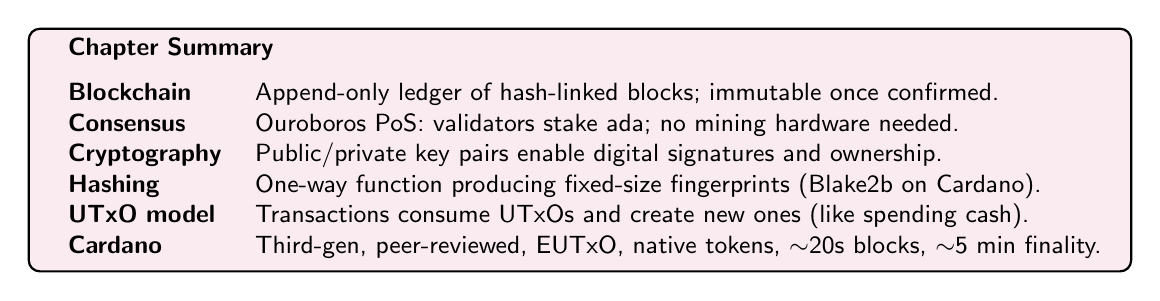
\begin{tikzpicture}
  \node[guidebox, fill=blockchaincolor, minimum width=14cm, minimum height=2.5cm,
        text width=13cm, align=left, font=\sffamily\small] {
    \textbf{Chapter Summary}\\[6pt]
    \begin{tabular}{@{}ll@{}}
    \textbf{Blockchain} & Append-only ledger of hash-linked blocks; immutable once confirmed.\\
    \textbf{Consensus}  & Ouroboros PoS: validators stake ada; no mining hardware needed.\\
    \textbf{Cryptography} & Public/private key pairs enable digital signatures and ownership.\\
    \textbf{Hashing}    & One-way function producing fixed-size fingerprints (Blake2b on Cardano).\\
    \textbf{UTxO model} & Transactions consume UTxOs and create new ones (like spending cash).\\
    \textbf{Cardano}    & Third-gen, peer-reviewed, EUTxO, native tokens, $\sim$20s blocks, $\sim$5 min finality.\\
    \end{tabular}
  };
\end{tikzpicture}
\end{center}
